Consider
\begin{equation}\label{eq:setdt}
g(\lambda) = \min_{C\subset V, C\neq \emptyset} \{ H(C) + \lambda\abs{C}\}
\end{equation}
where $H(C) = f(C) - \sum_{i\in C} f(\{i\})$, $f(C)$ is submodular, and $\abs{\cdot}, f\{i\}$ is modular.
Therefore the function to minimize in equation \eqref{eq:setdt} is submodular and standard algorithm can be
used to compute $g(\lambda)$.
Notice that $H(C)=0$ for $\abs{C}=1$.

The function defined in the above equation is piecewise linear about $\lambda$.
\begin{theorem}\label{thm:LastCriticalValue}
The largest turning point of $\gamma$ is equal to $\gamma_N$, which is the last critical value of info-clustering.
\end{theorem}
From the property of last critical value, it equals $\max_{C\subset V: \abs{C}>1}J_T(Z_C)$,
where $J_T(\cdot)$ is Watanabe's total correlation. Its definition is given as follows:
\begin{equation}
J_T(Z_C) = \frac{1}{\abs{C}-1} [\sum_{i\in C} f(\{i\}) - f(C)]
\end{equation}
The last line segment of $g(\lambda)$ is simply $\lambda$ itself.
\begin{proof}[Proof of theorem \ref{thm:LastCriticalValue}]
\begin{align*}
\gamma_N & = \max_{C\subset V: \abs{C}>1} J_T(Z_C) \\
& = \min\{\lambda : \lambda \geq \frac{-H(C)}{\abs{C}-1} \textrm{ for all $C\subset V$ and $\abs{C}>1$}\} \\
& = \min\{\lambda : \lambda \leq H(C)+\lambda\abs{C} \textrm{ for all $C\subset V$ and $\abs{C}>1$}\} \\
& = \min\{\lambda : \lambda \leq g(\lambda) \} \textrm{ holds for } \abs{C}=1
\end{align*}
\end{proof}

We give an example to illustrate $g(\lambda)$, consider four
uniformly distributed and independent Bernoulli random variables $X_a, X_b, X_c, X_d$ and $
Z_1 = (X_a, X_b), Z_2 = X_a, Z_3 = X_c, Z_4 = X_c, Z_5 = X_d$.

Let $V=\{1,2,3,4,5\}$ and $f(C) = H(\{Z_i |  i \in C \})$ for $C\subset V$.
For example $f(\{1\}) = 2, f(\{2\})=1, f(\{2,3\})=2$.
$g(\lambda)$ in this example is drawn in Fig \ref{fig:gLambda}.
\begin{figure}[!ht]
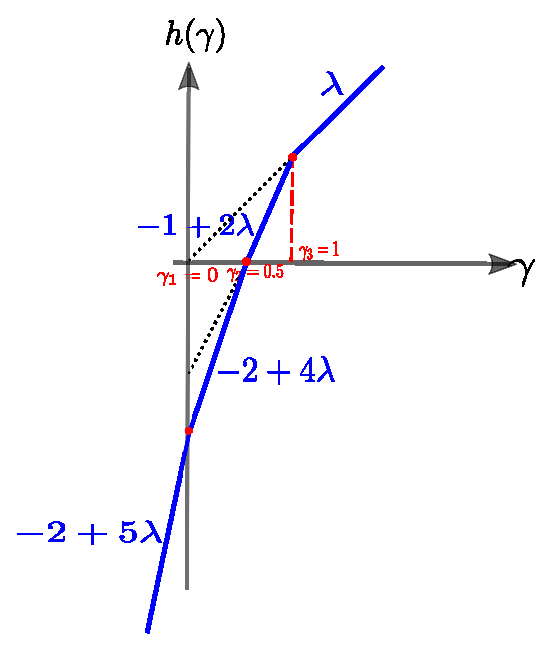
\includegraphics[width=6cm]{pic/dt2.eps}
\caption{$g(\lambda)$}\label{fig:gLambda}
\end{figure}
